\section{实验}\label{sec:experiments}

我们从四个方面评估该层：合成分支交叉处梯度的行为、Laplace 近似相对精确求积的精度、代数与松弛结果，以及在 LINEMOD 深度数据上构造的真实双模态代价。所有运行均为单进程 CPU 作业。

\subsection{实验设置与度量}\label{sec:metrics}

评估使用 $[-0.2,0.2]$ 上的 $81$ 点合成交叉网格，以及 $15$ 帧真实 LINEMOD 数据（$8$ 帧 \texttt{eggbox}、$7$ 帧 \texttt{glue}）。合成基准返回全部局部极小及沿分支的有限差分（FD）参考；一维标准型是唯一可以用稠密求积计算后验积分的设置。合成实例为构造而非拟合：$M(\theta)=M_{\rm sym}+\theta M_{\rm break}$，具有 $P$ 不变双井，$d(J_B-J_A)/d\theta|_{\theta=0}=2.0$，平移块固定且 $G\succ0$，种子为 20261127；枚举采用 $\mathbb{S}^3$ 上的批量阻尼 Newton，$128$ 个随机起点，$SO(3)$ 距离去重（阈值 $10^{-5}$ rad）与驻点过滤（$\|\nabla J\|\le10^{-8}$，$\lambda_{\min}(H_{\mathbb{S}^3})>10^{-8}$）。真实实例用真实内参把 BOP \texttt{mask\_visib} 内的深度像素反投影为方位向量，将每个方位分配给最近的网格顶点（KD 树），并以确定性 RANSAC（2.5 mm 内点带）选择主平面，参数为 $n_{\rm points}=900$、$n_{\rm starts}=384$、$\tau=0.01$、FD $h=10^{-4}$。

\textbf{梯度相对误差。} 以 $\phi=[\mathrm{vec}\,R(q);t^\star(q)]\in\mathbb{R}^{12}$ 计算 $\|\hat d\phi-d\phi_{\mathrm{FD}}\|_2/\|d\phi_{\mathrm{FD}}\|_2$，参考为沿分支的中心 FD（A、B 部分 $h=10^{-4}$，其余 $h=10^{-3}$；计时研究使用 Richardson 外推参考）。对全局打平处的硬 argmin，参考分支在 $\pm h$ 内切换，该项记为 N/A 而不以跳变填充；FD 自身的截断误差单独度量。

\textbf{MC 位姿散布。} 取 $20$ 次独立模态级 MC 均值（每次 $n=200$ 个样本）所得 $\phi$ 标准差向量的欧氏范数；平移块固定为 $D_{\text{scale}}=0.30$，故这是相对散布。B 部分每个 $\theta$ 使用 $n=400$；计时研究使用 $n=200$ 与 $3$ 个种子。

\textbf{位姿误差、ADD-S 与 ADD。} 旋转误差为真旋转上的测地角 $\arccos((\operatorname{tr}(R_{\rm est}^\top R_{\rm gt})-1)/2)$（度）；平移误差为 $\|t_{\rm est}-t_{\rm gt}\|$（米，BOP \texttt{cam\_t\_m2c} 以毫米计）。Laplace 估计为\textbf{投影弦均值} $R_{\rm Lap}=\mathrm{Proj}_{SO(3)}(\sum_kw_kR_k)$，$t_{\rm Lap}=\sum_kw_kt_k$。原始 9 维平均不正交，故对其套用测地公式得到 $58.28^\circ$ 并非旋转误差；投影均值上的中位数为 $44.24^\circ$，且 ADD-S 只对投影位姿有定义。ADD-S 变换 $1000$ 个查询顶点，并将每个点匹配到真值变换后\emph{完整}网格的最近顶点（$18{,}473$ 个 \texttt{eggbox} / $7{,}479$ 个 \texttt{glue} 顶点；三个查询子样本）：$\mathrm{ADD\text{-}S}=\frac{1}{|V|}\sum_{x\in V}\min_{y\in V_{\rm gt}}\|R_{\rm est}x+t_{\rm est}-(R_{\rm gt}y+t_{\rm gt})\|$。以 $1000$ 个真值顶点作匹配时，同子样本变体平均带有 $+1.1$ mm 的离散化下限（硬位姿），而 $1000$ 查询/稠密真值估计与全网格对全网格 ADD-S 相差 $0.51$ mm。ADD 使用同索引距离，仅作参考；由于 \texttt{eggbox}（物体 10）与 \texttt{glue}（物体 11）各具离散 $\sim180^\circ$ 对称性，ADD 会对对称等价位姿计入约物体直径量级的误差（$0.165$ m / $0.176$ m），故采用 ADD-S 更为合适。

\textbf{置信区间、偏差与派生量。} 对帧做百分位 bootstrap（位姿误差 $1000$ 次重采样，经典求解器 $2000$ 次）；成对偏差为相对硬 argmin 的逐帧差的均值。$15$ 帧下置信区间描述的是该固定帧集而非总体；对 MC，在 $20$ 个逐种子聚合值上做种子级 bootstrap 以分离种子噪声（聚合旋转误差的种子间标准差为 $1.011^\circ$）。耗时是每次层调用的 CPU 毫秒数（$20$ 次重复的中位数与 p95）。一维误差为 $|E_{\mathrm{Lap}}-E_{\mathrm{exact}}|$、其与 $\tau$ 之比、相对 $\tau$ 的双对数斜率与相对梯度误差；折叠误差为 $|Z_{\mathrm{Lap}}-Z_{\mathrm{exact}}|/Z_{\mathrm{exact}}$。SDP 量包括原始值、对偶 $\mu$、$\lambda_{\min}(Z)$、$10^{-6}$ 容差下的 $\operatorname{rank}(X^\star)$、$\lambda_1/\lambda_2$、间隙 $f^\star-\mu$，以及精确约束张成秩（21 $\to$ 20；上游 24 $\to$ 17；24 + 3 条行正交 $\to$ 20）。导数检验给出黎曼 Hessian、隐式 Jacobian 与 $\partial_\theta\log\det H$ 相对中心 FD 的相对误差。

\subsection{合成 6D 分支交叉}\label{sec:synthetic}

图~\ref{fig:p1summary} 以一幅图概括本文的四类结果：6D 交叉、实测 6D 折叠、真实 LINEMOD 双模态结构，以及 $10\times10$/$13\times13$ 分离。

\begin{figure*}[t]
\centering
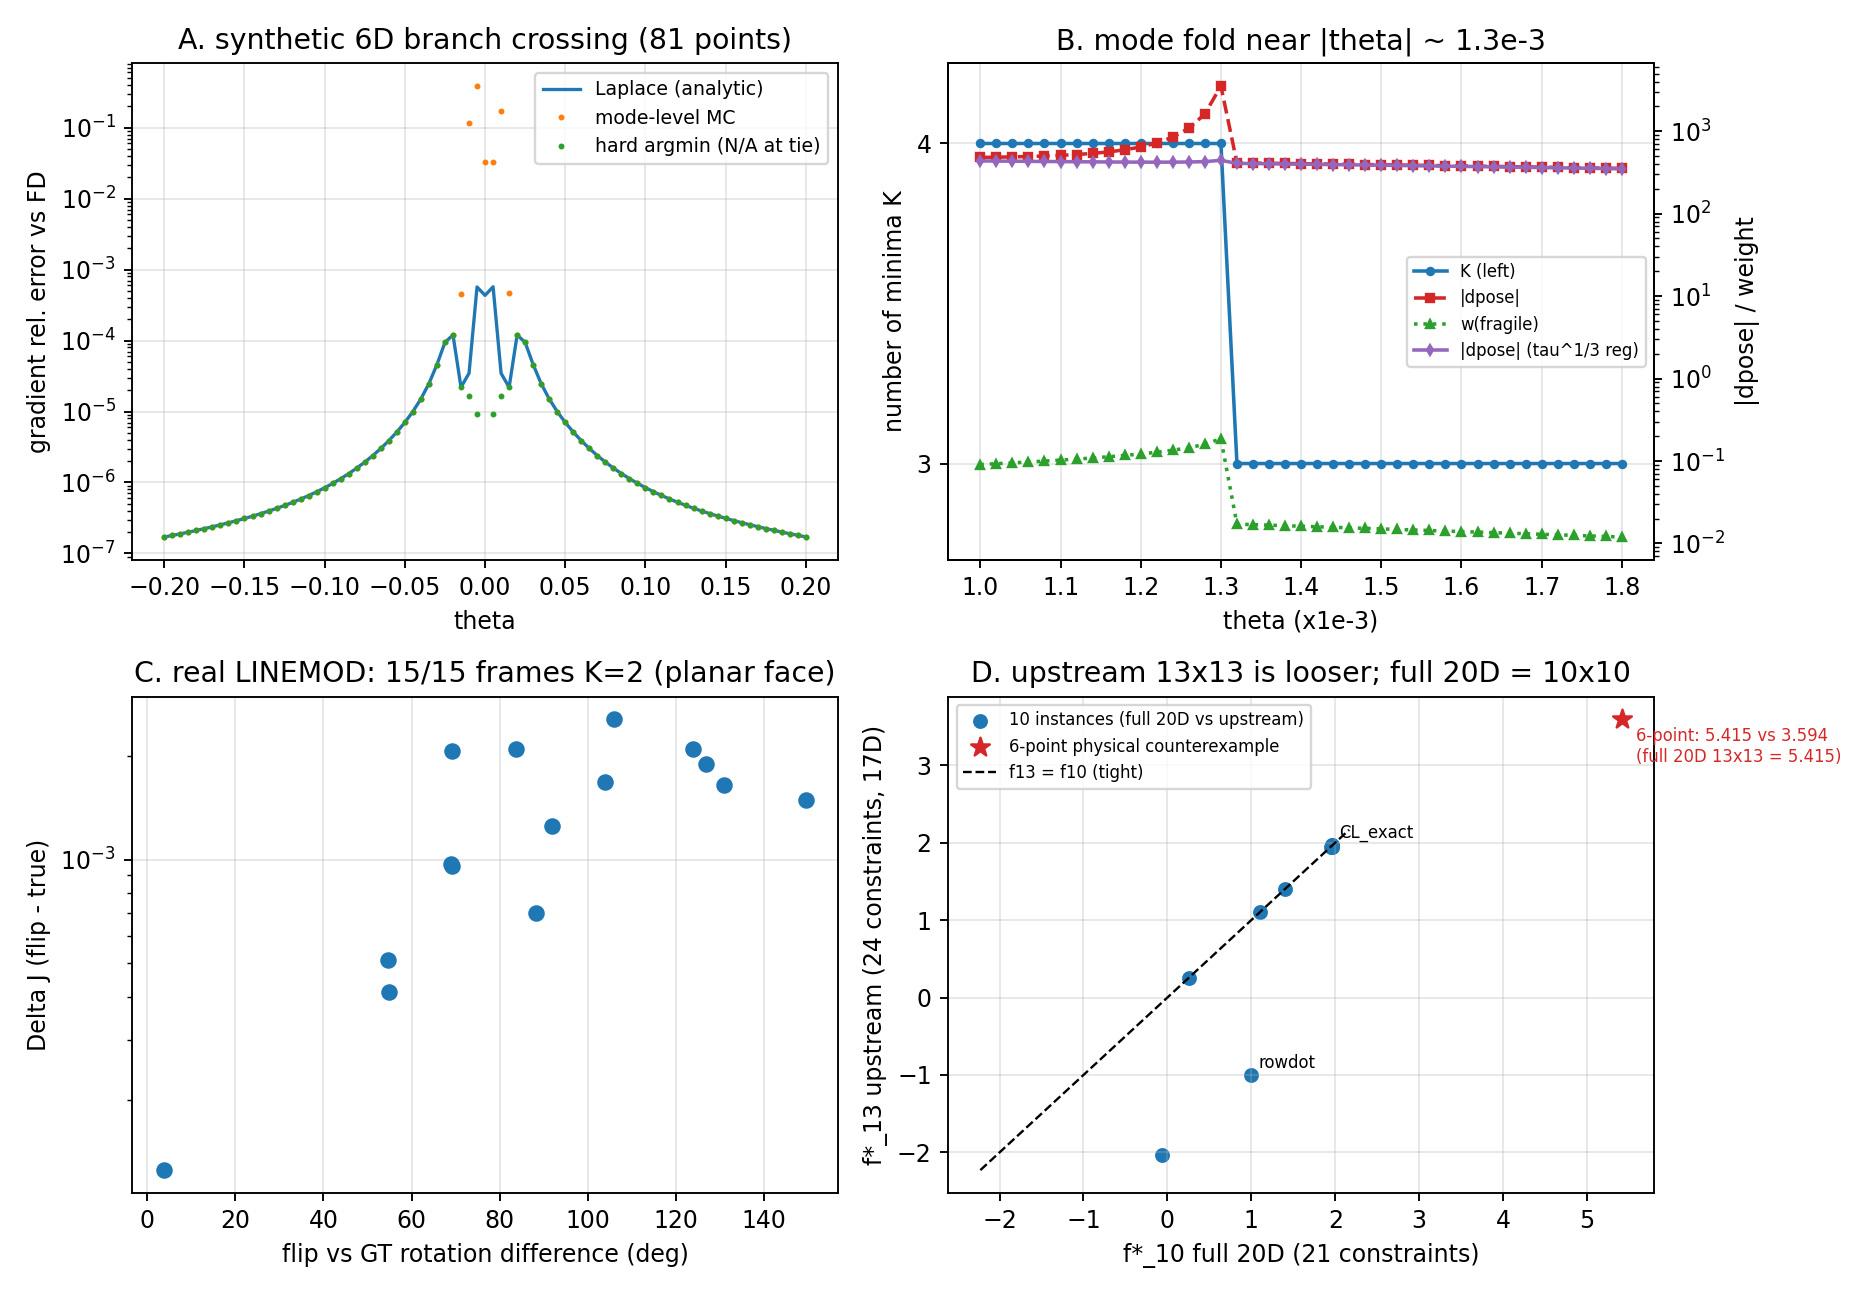
\includegraphics[width=0.92\textwidth]{p1_summary.png}
\caption{四类结果总览。\textbf{(A)} $81$ 点合成 6D 交叉上，解析 Laplace 层、模态级 MC 估计与硬 argmin 的梯度相对误差随 $\theta$ 的变化（交叉处为 N/A）；Laplace 曲线无跳变，硬映射有跳变。\textbf{(B)} $|\theta|\sim1.3\times10^{-3}$ 附近的实测 6D 折叠：极小个数 $K$、位姿映射跳变 $\|d\phi\|$（标准与 $\tau^{1/3}$ 正则化）以及脆弱模态的 Laplace 权重随 $\theta$ 的变化，横轴尺度为 $1.3\times10^{-3}$；模态在 $\theta_f$ 处消失，$\|d\phi\|$ 在该处尖峰。\textbf{(C)} 真实 LINEMOD 帧：目标间隙 $\Delta J$（翻转模态减真模态）与翻转-真值旋转差的关系；$15$ 帧均有 $K=2$。\textbf{(D)} $10$ 个 SDP 实例与 $8$ 个扰动上，上游 24 约束 $13\times13$ 值与完整 20 维 $10\times10$ 值的对比，六点物理反例（星号）将二者分开：$5.415$（完整 20 维）对 $3.594$（上游）。}
\label{fig:p1summary}
\end{figure*}

\begin{table}[t]
\centering
\caption{$81$ 点交叉网格各区间上解析 Laplace 层、模态级 MC 基线与硬 argmin 的梯度相对误差，以及 MC 位姿散布（$\tau=0.01$，FD $h=10^{-4}$，模态级 MC $n=200$、$20$ 个种子，CPU）。每项为区间内网格点的中位数。$\theta=0$ 处的硬 argmin 项为 N/A，因为全局分支在 $\pm h$ 内切换。}
\label{tab:main6d}
\footnotesize
\setlength{\tabcolsep}{4pt}
\begin{tabular}{@{}l r l l l l@{}}
\toprule
区间 & $n$ & Laplace & MC & 硬 argmin & MC 标准差\\
\midrule
远区 & 61 & 4.74e-07 & 4.74e-07 & 4.74e-07 & 2.76e-16\\
近区 & 19 & 3.46e-05 & 9.40e-05 & 2.23e-05 & 2.89e-16\\
交叉点 & 1 & 4.34e-04 & 3.26e-02 & N/A & 1.07e-01\\
\bottomrule
\end{tabular}
\end{table}

网格包含 $61$ 个远区点、$19$ 个近区点与单个交叉点（名义边界 $|\theta|=0.05$ 与 $0.005$）。由此可得三点观察。

\begin{enumerate}
\item \textbf{远离交叉处三种方法一致。} 远区三种方法的相对误差中位数均为 $4.74\times10^{-7}$，MC 位姿散布中位数为 $2.76\times10^{-16}$：全局模态几乎承载全部 Laplace 质量，采样器只看到一个模态。
\item \textbf{Laplace 的优势仅出现在交叉处。} 近区硬 argmin 仍有定义，且中位误差最小（$2.23\times10^{-5}$），优于 Laplace 与 MC；MC 散布中位数为 $2.89\times10^{-16}$，但逐点最大值为 $3.41\times10^{-2}$。$\theta=0$ 处硬 argmin 项为 N/A，Laplace 项受 FD 限制（见下文），MC 误差为 $3.26\times10^{-2}$，位姿散布为 $1.07\times10^{-1}$。
\end{enumerate}

\textbf{$4.34\times10^{-4}$ 是 FD 截断而非方法误差。} 对 Richardson 外推 FD，$\theta=0$ 处为 $1.8\times10^{-7}$，而对 $h=10^{-4}$ 的普通中心 FD 为 $4.3\times10^{-4}$；序列 $4.34\times10^{-8}$（$h=10^{-6}$）、$4.34\times10^{-6}$（$h=10^{-5}$）、$4.34\times10^{-4}$（$h=10^{-4}$）说明了同一点。近区行同样受 FD 限制：$\theta=0.01$ 处 $h=10^{-6}$ 给出 $3.46\times10^{-9}$，而 $h=10^{-4}$ 给出 $3.46\times10^{-5}$。对 $|\theta|\ge0.05$，$h=10^{-5}$ 的误差至多 $7.0\times10^{-8}$。解析梯度在交叉处与 Richardson FD 一致到 $1.8\times10^{-7}$，而不是 $4\times10^{-4}$。

\textbf{硬 argmin 是阶跃映射，Laplace 映射不是。} 随 $\delta\to0$（$\delta=10^{-3},10^{-4},10^{-5}$），$\theta=0$ 两侧的硬位姿跳变保持 $2.86$，而 Laplace 跳变线性衰减（$9.73\times10^{-1}$、$1.00\times10^{-1}$、$1.00\times10^{-2}$），FD 斜率为 $\approx502$，即真实导数。在中心 FD 有定义处，硬映射与 Laplace 一样自洽（非切换情形的中位数为 $1.2\times10^{-4}$），但在恰好交叉的情形中有一半在 $\pm h$ 内切换分支。图~\ref{fig:maintable} 给出逐点误差与 MC 散布。

\begin{figure}[t]
\centering
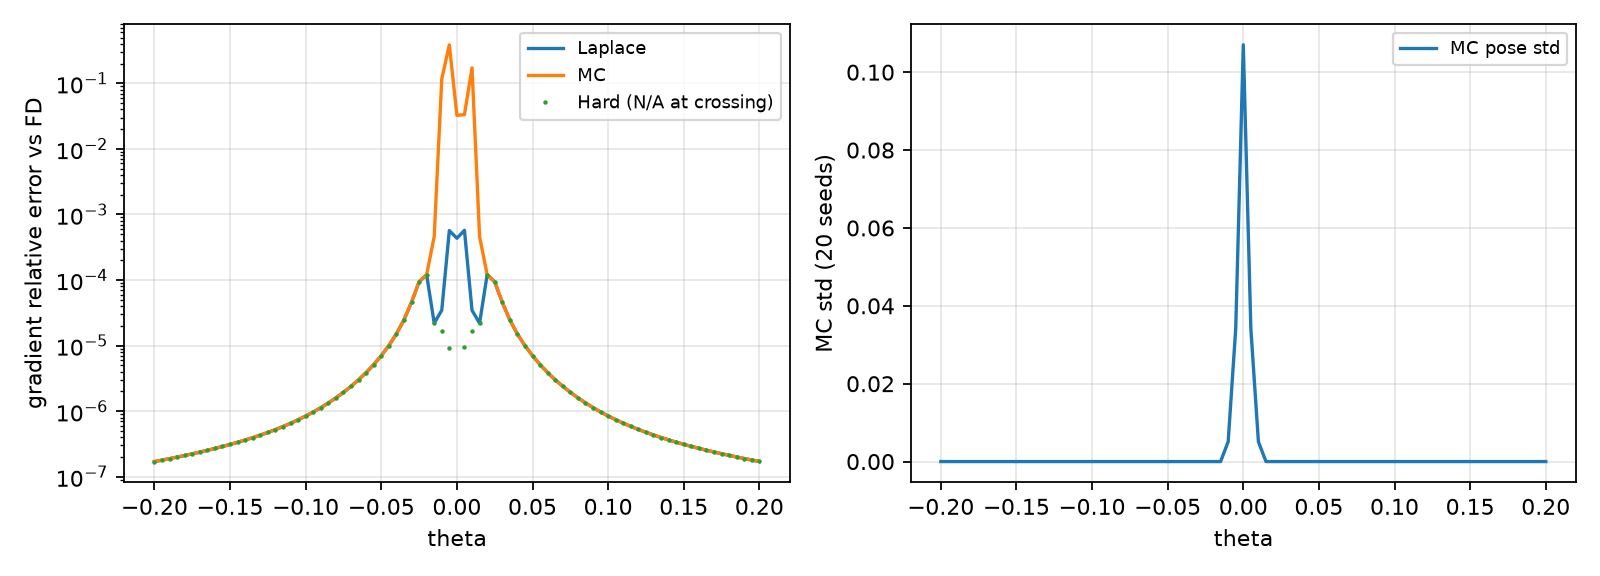
\includegraphics[width=\columnwidth]{main_table.png}
\caption{$81$ 点 6D 交叉网格上的主表诊断。左：解析 Laplace 层（蓝）、模态级 MC 估计（橙）与硬 argmin（绿点；在 FD 参考切换分支的精确交叉处为 N/A）相对沿分支 FD 的梯度误差。右：$20$ 个种子上的 MC 位姿标准差，除 $\theta=0$ 附近窄窗外基本为零。}
\label{fig:maintable}
\end{figure}

\textbf{MC 基线无偏，但在固定预算下噪声较大。} 对同一平滑目标，$n=200\times3$ 个种子给出的逐种子梯度相对误差中位数为 $0.05$（$20$ 种子均值 $7.7\times10^{-3}$），各鲁棒性条件下位姿标准差中位数为 $0.09$，而解析 Laplace 梯度相对 Richardson 参考为 $9.3\times10^{-8}$。这是模态级采样的实测方差代价。

\textbf{模态数与折叠。} 网格上模态数为 $K\in\{1,2,3,4\}$（$K=1$ 有 $30$ 点，$K=2$ 有 $38$ 点，$K=3$ 有 $12$ 点，交叉点为 $K=4$）；这些是上述过滤后的多起点 Newton 返回的局部极小，而非认证根数。光滑性结论限于 $\theta=0$ 与 $|\theta|\lesssim1.3\times10^{-3}$：次极小只在此范围内存在，并在折叠处消失，Laplace 映射在该处不连续（第~\ref{sec:fold6d}~节）。

\subsection{一维精确后验：Laplace 误差为 \texorpdfstring{$O(\tau)$}{O(tau)}}\label{sec:onepd}

\begin{table*}[t]
\centering
\caption{曲率不等的一维标准型中精确后验与双模态 Laplace 的对比（$c=0.25$；$g=0$ 时两个极小位于 $x=\pm1$，曲率为 5 与 3）。$E$ 为 $x$ 的后验均值；误差相对 $[-3,3]$ 上 $2{,}000{,}001$ 点梯形求积。能量为无量纲量，$\Delta J=6.16\times10^{-32}$ 为数值零。}
\label{tab:1d}
\footnotesize
\setlength{\tabcolsep}{5pt}
\begin{tabular}{@{}l l l l l l l l@{}}
\toprule
情形 & $\tau$ & $\Delta J$ & $E_{\mathrm{exact}}$ & $E_{\mathrm{Lap}}$ & $|{\rm err}|$ & $|{\rm err}|/\tau$ & 相对梯度误差\\
\midrule
交叉 & 0.05 & 6.16e-32 & -0.125102 & -0.127017 & 1.92e-03 & 3.83e-02 & 1.77e-02\\
交叉 & 0.02 & 6.16e-32 & -0.126275 & -0.127017 & 7.42e-04 & 3.71e-02 & 6.93e-03\\
交叉 & 0.01 & 6.16e-32 & -0.126649 & -0.127017 & 3.67e-04 & 3.67e-02 & 3.44e-03\\
交叉 & 0.005 & 6.16e-32 & -0.126834 & -0.127017 & 1.83e-04 & 3.66e-02 & 1.71e-03\\
分离 & 0.05 & 4.01e-01 & -1.024203 & -1.031750 & 7.55e-03 & 1.51e-01 & 2.77e-02\\
分离 & 0.02 & 4.01e-01 & -1.029356 & -1.032296 & 2.94e-03 & 1.47e-01 & 1.27e-02\\
分离 & 0.01 & 4.01e-01 & -1.030838 & -1.032296 & 1.46e-03 & 1.46e-01 & 6.27e-03\\
分离 & 0.005 & 4.01e-01 & -1.031570 & -1.032296 & 7.26e-04 & 1.45e-01 & 3.12e-03\\
\bottomrule
\end{tabular}
\end{table*}

期望值误差按 $O(\tau)$ 缩放：交叉处双对数斜率为 1.066，分离盆为 1.036；交叉处 $|{\rm err}|/\tau$ 保持在 $3.66$--$3.83\times10^{-2}$，分离时为 $1.45$--$1.51\times10^{-1}$。梯度误差在表中所列行上随 $\tau$ 单调下降；梯度余项以数值方式检验，而非证明。

\subsection{折叠合并与 \texorpdfstring{$\tau^{1/3}$}{tau^(1/3)} 正则化子}\label{sec:fold1d}

\begin{table*}[t]
\centering
\caption{$\tau=0.01$ 时标准 Laplace 与 $\tau^{1/3}$ 正则化体积因子的对比，$J=x^4/4-ax^2/2$；精确配分由 $[-3.5,3.5]$ 上 $2{,}000{,}001$ 点梯形求积给出。$H=2a$ 为极小处曲率，势垒为 $a^2/4$。}
\label{tab:fold}
\scriptsize
\setlength{\tabcolsep}{2.5pt}
\begin{tabular}{@{}l l l l l l l l@{}}
\toprule
$a$ & $H$ & 势垒 & $Z_{\mathrm{exact}}$ & $Z_{\mathrm{Lap}}$ & Lap 相对误差 & $Z_{\mathrm{reg}}$ & reg 相对误差\\
\midrule
0.50 & 1.00e+00 & 6.25e-02 & 2.6976e+02 & 2.5969e+02 & 3.73e-02 & 2.3556e+02 & 1.27e-01\\
0.20 & 4.00e-01 & 1.00e-02 & 2.3994e+00 & 2.1547e+00 & 1.02e-01 & 1.7371e+00 & 2.76e-01\\
0.10 & 2.00e-01 & 2.50e-03 & 1.2349e+00 & 1.4394e+00 & 1.66e-01 & 9.9871e-01 & 1.91e-01\\
0.05 & 1.00e-01 & 6.25e-04 & 9.7810e-01 & 1.6876e+00 & 7.25e-01 & 9.5017e-01 & 2.86e-02\\
0.02 & 4.00e-02 & 1.00e-04 & 8.6986e-01 & 2.5318e+00 & 1.91e+00 & 1.0019e+00 & 1.52e-01\\
0.01 & 2.00e-02 & 2.50e-05 & 8.3916e-01 & 3.5538e+00 & 3.24e+00 & 1.0358e+00 & 2.34e-01\\
\bottomrule
\end{tabular}
\end{table*}

当 $a\to0$ 时两个极小与鞍点合并，$H\to0$，标准体积因子 $1/\sqrt{H}$ 发散：相对误差从 $a=0.5$ 的 $3.73\times10^{-2}$ 增至 $a=0.02$ 的 $1.91$ 与 $a=0.01$ 的 $3.24$。把 $H$ 换成 $H+\tau^{1/3}$ 后，两个最小 $a$ 处的误差降为 $1.52\times10^{-1}$ 与 $2.34\times10^{-1}$，但并非一致更优：$a=0.5$ 处反而更差（$1.27\times10^{-1}$ 对 $3.73\times10^{-2}$）。正则化形式刻画了合并区域的 $\tau^{1/3}$ 缩放，但并非处处可直接替代。

\subsubsection{实测 6D 折叠}\label{sec:fold6d}

6D 合成映射在交叉附近存在真实折叠。次极小仅在 $|\theta|\lesssim1.3\times10^{-3}$ 时存在（精细折叠扫描给出模态消失点 $\theta_f=1.31\times10^{-3}$，较粗的鲁棒性扫描将其括在 $\approx1.4\times10^{-3}$）；接近折叠时其 $3\times3$ Hessian 行列式降到 $3.35\times10^{-1}$，Laplace 权重从 $0.09$ 升到 $0.187$（该行列式处为 $0.122$），随后模态消失（$K$ 从 4 降到 3）。跨过折叠时位姿映射在一步 $2\times10^{-5}$ 上跳变 $0.31$（在网格加密下保持不变，即真实不连续），$\|d\phi\|$ 峰值达 $3529$，而远离折叠处中位数为 $379$；有效 FD 斜率可达 $1.5\times10^4$。更小的 $\tau$ 或更多起点都不能消除它：$n_{\rm starts}\ge32$ 与 $1024$ 起点的 $K$ 中位数一致（$64$ 个起点在扫描中复现完整模态集），而 $n_{\rm starts}=16$ 在 $10\%$ 的独立抽样中漏掉脆弱模态，一次漏检使位姿最多偏移 $28\%$、梯度最多偏移 $97\%$。因此光滑性与 $O(\tau)$ 精度结论限于 $\theta=0$ 与 $|\theta|\lesssim1.3\times10^{-3}$；多模态 Laplace 映射在极小产生或消失处不连续。

\textbf{折叠的部分修正。} 把 $\det H$ 换成 $\det(H+\epsilon I)$，$\epsilon=\tau^{1/3}$（即上述一维规则，其导数仍为闭式 $\operatorname{tr}((H+\epsilon I)^{-1}\dot H)$），基本消除了\emph{导数}奇异性：$\theta=1.30\times10^{-3}$ 处标准 $\|d\phi\|$ 为 $3529$，正则化后为 $443$；近折叠梯度误差从 $2.90\times10^{-1}$ 降到 $1.19\times10^{-2}$（因子 24）；远离折叠处（$\theta=0.1,0.02$）两种变体在打印精度内一致。它不能消除极小消失导致的\emph{数值}不连续：跨折叠位姿跳变只从 $0.309$ 降到 $0.107$，$K$ 仍从 4 变到 3。因此 Hessian 正则化是折叠邻域的低成本缓解，而跨折叠的连续性结论需要第~\ref{sec:discussion}~节的 Scorer 延拓，或对合并对做局部数值积分。

\subsection{旋转 SDP 证书与三段式 \texorpdfstring{$10\times10$/$13\times13$}{10x10/13x13} 关系}\label{sec:results_sdp}

\begin{table}[t]
\centering
\caption{构造的 $10\times10$ 旋转 SDP 的数值证书（Choi--Lam 四次型加 $2I$；SCS）。间隙为 $f^\star-\mu$，其中 $f^\star=2$ 为四次型在 $\mathbb{S}^3$ 上的解析极小，$\mu$ 为认证对偶值。}
\label{tab:sdp_cert}
\scriptsize
\setlength{\tabcolsep}{3pt}
\begin{tabular}{@{}p{4.6cm} l@{}}
\toprule
量 & 值\\
\midrule
$f^\star$（解析，$C\ge0$，$C(e_0)=0$） & 2.0\\
SDP 原始值 & 1.9658119658\\
对偶 $\mu$ & 1.9658119658\\
对偶证书的 $\lambda_{\min}(Z)$ & $-1.79\times10^{-11}$\\
认证间隙 $f^\star-\mu$ & 0.034188\\
$10^{-6}$ 容差下的 $\operatorname{rank}(X^\star)$ & 6\\
$\lambda_1/\lambda_2$ & 1.451\\
多起点 QPEP 极小（独立校核） & 2.00186\\
具有正间隙的随机扰动 & 8 / 8（0.0453--0.0782）\\
21 条 $SO(3)$ 约束的秩 & 20\\
二次消没理想的维数 & 20\\
\bottomrule
\end{tabular}
\end{table}

$10\times10$ 实例的原始值、对偶值与间隙在打印精度内相互一致；间隙为 $0.034188034\ldots$。这是本文构造（例~\ref{ex:choilam}）。定理~\ref{thm:thirteen} 给出与已发布 $13\times13$ 实现的三段式关系，下述度量分别对应其中每一层。

\begin{table*}[t]
\centering
\caption{上游 24 约束 $13\times13$ 松弛在一般情况下严格松于完整 20 维 $10\times10$ 松弛。$f^\star_{10}$ 为 $10\times10$ 值，$f^\star_{13,\mathrm{up}}$ 为已发布 24 约束实现的值（17 维张成空间）；\texttt{CL\_exact} 为构造的 Choi--Lam 实例，\texttt{rowdot} 为构造的反例。对 \texttt{CL\_exact} 与 \texttt{p6\_data}，真实差值分别为 $3.7\times10^{-11}$ 与 $-2.9\times10^{-10}$，低于六位小数的显示精度。}
\label{tab:13v10}
\footnotesize
\setlength{\tabcolsep}{6pt}
\begin{tabular}{@{}l l l l l l@{}}
\toprule
实例 & $f^\star_{10}$ & $f^\star_{13,\mathrm{up}}$ & $f^\star_{10}-f^\star_{13,\mathrm{up}}$ & 秩 $X_{10}^\star$ & 秩 $X_{13,\mathrm{up}}^\star$\\
\midrule
\texttt{CL\_exact} & 1.965812 & 1.965812 & 3.7e-11 & 6 & 6\\
\texttt{CL\_pert0} & 1.962860 & 1.960078 & 2.8e-03 & 6 & 5\\
\texttt{CL\_pert5} & 1.964571 & 1.950275 & 1.4e-02 & 6 & 4\\
\texttt{rowdot} & 1.000000 & -1.000000 & 2.00 & 10 & 7\\
\texttt{rowdot\_gen} & -0.060192 & -2.029230 & 1.97 & 1 & 4\\
\texttt{p6\_data} & 0.252326 & 0.252326 & 0.0 & 1 & 1\\
\bottomrule
\end{tabular}
\end{table*}

\textbf{解释。} Choi--Lam 等式是对称性的巧合：其上游最优解落在行正交面上，故 $f^\star_{13,\mathrm{up}}=f^\star_{10}=1.9658119658$，两侧秩均为 6，行点积残差至多 $8.8\times10^{-15}$。在八个 $10^{-2}$ 量级的对称破缺扰动后，$8/8$ 个实例满足 $f^\star_{13,\mathrm{up}}<f^\star_{10}$，差值为 $2.5\times10^{-3}$--$1.4\times10^{-2}$，$\operatorname{rank}(X^\star_{13,\mathrm{up}})\in\{4,5\}$ 而 $\operatorname{rank}(X^\star_{10})=6$，上游最优处的 $\max|r_a\cdot r_b|$ 为 $0.59$--$0.88$。构造目标 $Q=-r_1\cdot r_2+\tfrac14I$ 隔离出该机制：它在完整 20 维可行集上是常数 1（$f^\star_{10}=1.000000$），而在上游可达 $-1.000000$（间隙 $2.00$），在 $10^{-2}$ 扰动后仍为 $1.97$。这些度量对应定理~\ref{thm:thirteen} 的第 (2) 层而非第 (1) 层。

\begin{table}[t]
\centering
\caption{区分上游 $13\times13$ 松弛与完整 20 维松弛的六点物理 3D--3D 反例。构造：$p_i=\pm e_1,\pm e_2,\pm e_3$，$y_i=\varepsilon p_i$，$\varepsilon=0.05$；共享矩阵权重 $W$ 满足 $W_{11}=W_{22}=W_{33}=1$、$W_{12}=W_{21}=-0.6$（特征值 $0.4,1.0,1.6>0$），$N=6$，故 $D=0$、$G=6W\succ0$；真值旋转 $R^\star=I_3$ 唯一。中间一列秩由第 (1) 层得到；解析列显式给出秩 1 与 4。}
\label{tab:6point}
\scriptsize
\setlength{\tabcolsep}{3pt}
\begin{tabular}{@{}p{4.1cm} l l@{}}
\toprule
量 & 数值 & 解析\\
\midrule
$f^\star_{10}$（21 条约束，精确秩 20） & 5.41500000 & 5.41500000\\
$f^\star_{13,\mathrm{full}}$（24 + 3 条行正交 = 27 条约束，完整 20 维） & 5.41500000 & 5.41500000\\
$f^\star_{13,\mathrm{up}}$（24 条约束，17 维张成） & 3.59431373 & 3.59430886\\
$f^\star_{10}-f^\star_{13,\mathrm{up}}$ & 1.82068627 & 1.82069114\\
$X^\star_{10}$ / $X^\star_{13,\mathrm{full}}$ / $X^\star_{13,\mathrm{up}}$ 的秩 & 1 / 1 / 4 & 1 / 1 / 4\\
$f_{\rm nonconv}-f^\star_{10}$ & $-8.38\times10^{-13}$ & 0\\
$f_{\rm nonconv}-f^\star_{13,\mathrm{full}}$ & $-3.38\times10^{-13}$ & 0\\
$f_{\rm nonconv}-f^\star_{13,\mathrm{up}}$ & 1.820686 & 1.820691\\
\bottomrule
\end{tabular}
\end{table}

\textbf{该实例为何能区分两者。} 由于 $\pm p_i$ 成对相消，$D=\mathbf{0}$，代价为
\begin{equation}
\begin{split}
J(R,t)={}&2\,\mathrm{tr}(WRR^\top)-4\varepsilon\,\mathrm{tr}(WR)\\
&+2\varepsilon^2\mathrm{tr}(W)+6t^\top Wt .
\end{split}
\label{eq:sixpoint}
\end{equation}
唯一涉及行正交性的项是 $2\,\mathrm{tr}(WRR^\top)=2(\|r_1\|^2+\|r_2\|^2+\|r_3\|^2-1.2\,r_1^\top r_2)$。在完整 20 维约束下，$r_1^\top r_2=0$ 使其成为常数 $6$，而 $-4\varepsilon\,\mathrm{tr}(WR)$ 在 $R=I$ 处取极小，值为 $6(1-\varepsilon)^2=5.415$，故 $f^\star_{10}=f^\star_{13,\mathrm{full}}=f^\star_{\mathrm{QPEP}}=5.41500000$，秩为 1，SCS 水平下间隙为零。上游缺少 $r_1^\top r_2=0$，松弛可取 $\langle r_1^\top r_2\rangle>0$，从而降到 $f^\star_{13,\mathrm{up}}=3.59431373$，秩为 4。

\textbf{解析列中 $4.9\times10^{-6}$ 的差异。} SCS（$\varepsilon=10^{-11}$）给出 $3.59431373$，CLARABEL 给出 $3.59431371$（一致到 $2\times10^{-8}$）；精确有理对偶证书（精确有理 LDU，$\eta=10^{-11}$；最小主元 $1.0\times10^{-11}$，mpmath 60 位 $\lambda_{\min}=+8.0\times10^{-12}$）给出严格下界 $f^\star_{13,\mathrm{up}}\ge3.594313732834$。解析值 $3.59430886$ 比该下界低 $4.87\times10^{-6}$，故不可能是所述 24 约束 SDP 的最优值；$36$ 种自然变体（缩放、子集、布局、归一化、$t$ 块与求解器容差）在 $10^{-8}$ 内都无法复现它，最接近的相差 $4.1\times10^{-6}$。求解器值 $3.5943137\ldots$ 与间隙 $1.8206863\ldots$ 才与该下界一致。定性分离（间隙 $1.82$，秩 $1$ 对 $>1$）不受影响；$\operatorname{rank}(X^\star_{13,\mathrm{up}})$ 在 $10^{-5}$ 阈值下为 $4$，在 $10^{-6}$ 下为 $6$。由于该实例是真实的矩阵加权 3D--3D 代价，Choi--Lam 可实现性问题不适用：间隙是已发布约束集的性质，而三条缺失的行正交约束就是全部原因。

\subsection{导数检验与根计数}\label{sec:rootcount}

\begin{table}[t]
\centering
\caption{反向传播与闭式 $\partial_\theta\log\det H$ 的数值检验。除标注“绝对”外，各项均为相对误差。}
\label{tab:backward}
\scriptsize
\setlength{\tabcolsep}{3pt}
\begin{tabular}{@{}p{3.85cm} p{3.9cm}@{}}
\toprule
检验 & 值\\
\midrule
$E(q)$ 正交性误差 & 1.14e-16\\
$E(q)^\top q$ 误差 & 4.41e-18\\
Euler 恒等式绝对误差 & 5.33e-15\\
黎曼 Hessian，解析对 FD & 9.63e-08\\
隐式 $\partial q^\star/\partial\theta$ 对 FD & 1.51e-07\\
隐式 $\partial t^\star/\partial\theta$ 对 FD & 4.58e-08\\
对映误差（$E$、$H$、$\partial q^\star$、$\partial R$） & 0（精确）\\
Laplace 积分相对误差（$\mathbb{S}^3$ 上的图卡），$\tau=0.2/0.1/0.05/0.025$ & 8.26e-02 / 3.81e-02 / 1.86e-02 / 9.25e-03\\
Laplace 误差对 $\tau$ 的双对数斜率 & 1.05\\
闭式 $\partial_\theta\log\det H$ 对 FD，$5$ 次试验 & 1.65e-09 -- 8.84e-09\\
\quad（最大绝对误差） & 1.59e-09\\
闭式 \texttt{dlogdetH\_dtheta} 对 \texttt{dlogdet\_exact}（修正后） & 8.9e-16\\
闭式 \texttt{dlogdetH\_dtheta} 对沿分支 FD（修正后） & 1.8e-9\\
回归检验：\texttt{dE}/\texttt{dH}/\texttt{dq} & 2.9e-11 / 1.6e-8 / 2.5e-10\\
\bottomrule
\end{tabular}
\end{table}

反向检验在 FD 精度内确认定理~\ref{thm:implicit}；它们并不认证根集。Laplace 常数检验给出斜率 1.05，与定理~\ref{thm:laplace} 的 $O(\tau)$ 结论一致，与精确旋转积分不一致。闭式 $\log\det$ 导数与独立精确导数一致到 $8.9\times10^{-16}$，与沿分支 FD 一致到 $1.8\times10^{-9}$，五次试验中与 FD 一致到 $9\times10^{-9}$ 或更好；回归检验固定 \texttt{dE}/\texttt{dH}/\texttt{dq} 为 $2.9\times10^{-11}$/$1.6\times10^{-8}$/$2.5\times10^{-10}$。

\textbf{根计数与枚举。} 在射影驻点系统上运行全次数同伦，覆盖四个仿射图卡，使用批量复预测-校正与残差校验并集，在 $4/4$ 个实例上找到 \textbf{40 个复射影根}——三个随机对称 $M$ 与 6D 实例 $M(0)$——最大图卡残差 $7.1\times10^{-15}$，每个实例 5.3--8.0 s。每个射影根对应带 $\pm$ 双覆盖的 80 个仿射根。实根情形随实例变化：实射影根为 $26/12/12/20$，实局部极小为 $5/2/2/4$；复根数是通用的（QPEP 作用矩阵界 40），实根数是实例性质。这确认了第~\ref{sec:cert}~节“至多 40 个候选复根”的说法，并认证了代数系统，但不认证 E1/E8 使用的多起点 Newton 枚举器。该枚举器仅在假设 (A2) 下精确：相对 $1024$ 起点参考，$n_{\rm starts}\ge64$ 在扫描中复现模态集，$32$ 与 $K$ 中位数一致，而 $n_{\rm starts}=16$ 在 $10\%$ 的独立抽样中漏掉脆弱模态，故第~\ref{sec:synthetic}~节的模态数是真实计数的下界。\label{sec:enumeration}

\subsection{消融实验}\label{sec:ablations}

\textbf{A. 温度。} 表~\ref{tab:tau} 给出精确 logdet Laplace 层在交叉处、近交叉处与远离交叉处的梯度相对误差。

\begin{table}[t]
\centering
\caption{$\tau$ 扫描（梯度相对误差）。}
\label{tab:tau}
\footnotesize
\setlength{\tabcolsep}{4pt}
\begin{tabular}{@{}l l l l l@{}}
\toprule
$\theta$ & $\tau=0.05$ & 0.02 & 0.01 & 0.005\\
\midrule
+0.000 & 1.20e-03 & 5.84e-04 & 4.34e-04 & 1.51e-03\\
+0.010 & 1.29e-05 & 1.07e-04 & 3.46e-05 & 1.64e-05\\
-0.010 & 1.29e-05 & 1.06e-04 & 3.46e-05 & 1.63e-05\\
+0.100 & 8.47e-07 & 8.46e-07 & 8.46e-07 & 8.46e-07\\
-0.100 & 8.43e-07 & 8.42e-07 & 8.42e-07 & 8.42e-07\\
\bottomrule
\end{tabular}
\end{table}

交叉处 $\tau=0.01$ 时误差最小，$\tau=0.005$ 时回升，这与两个模态近简并时 FD 参考变得不可靠相符；远离交叉处误差约为 $\approx8.5\times10^{-7}$，且与 $\tau$ 无关。

\textbf{B. 体积因子。} 表~\ref{tab:volume} 比较闭式 $\log\det$ 导数、切空间 FD 与从权重中去掉体积因子三种变体。

\begin{table}[t]
\centering
\caption{体积因子变体。\texttt{exact} 为第~\ref{sec:laplace}~节的闭式，\texttt{numeric} 为切空间 FD，\texttt{none} 从权重中去掉 $\tfrac12\log\det H_k$；\emph{位姿差} 与 \emph{梯度差} 为 12 维向量相对 \texttt{exact} 的欧氏范数。}
\label{tab:volume}
\scriptsize
\setlength{\tabcolsep}{3pt}
\begin{tabular}{@{}l l l l l@{}}
\toprule
$\theta$ & 变体 & 梯度相对误差 & 位姿差 & 梯度差\\
\midrule
+0.000 & exact & 4.34e-04 & 0.00e+00 & 0.00e+00\\
+0.000 & numeric & 4.34e-04 & 0.00e+00 & 2.22e-08\\
+0.000 & none & 3.75e-04 & 6.47e-02 & 5.34e+01\\
+0.010 & exact & 3.46e-05 & 0.00e+00 & 0.00e+00\\
+0.010 & numeric & 3.46e-05 & 0.00e+00 & 1.22e-11\\
+0.010 & none & 3.86e-05 & 7.77e-04 & 4.38e-01\\
-0.010 & exact & 3.46e-05 & 0.00e+00 & 0.00e+00\\
-0.010 & numeric & 3.46e-05 & 0.00e+00 & 1.89e-11\\
-0.010 & none & 3.86e-05 & 7.79e-04 & 4.39e-01\\
\bottomrule
\end{tabular}
\end{table}

在交叉处去掉体积因子几乎不改变梯度相对误差，但使平滑位姿改变 $6.47\times10^{-2}$、梯度绝对范数改变 $5.34\times10^{1}$；近交叉处梯度改变 $0.44$。因此该因子对平滑映射并非装饰性的，闭式与切空间 FD 一致到 $2.22\times10^{-8}$ 或更好。

\textbf{C. Top-$K$ 模态截断。} 表~\ref{tab:topk} 只保留权重最高的 $K$ 个模态，并与全部模态之和比较。

\begin{table}[t]
\centering
\caption{Top-$K$ 模态截断（参考：全部模态）。}
\label{tab:topk}
\footnotesize
\setlength{\tabcolsep}{4pt}
\begin{tabular}{@{}l l l l@{}}
\toprule
$\theta$ & $K$ & 位姿差 & 梯度差\\
\midrule
+0.000 & 1 & 1.44e+00 & 4.99e+02\\
+0.000 & 2 & 1.05e-01 & 6.83e+01\\
+0.000 & 3 & 7.95e-02 & 4.93e+01\\
+0.000 & 4 & 0.00e+00 & 0.00e+00\\
+0.010 & 1 & 2.72e-03 & 1.98e+00\\
+0.010 & 2 & 3.02e-05 & 2.65e-02\\
+0.010 & 3 & 0.00e+00 & 0.00e+00\\
+0.010 & 4 & 0.00e+00 & 0.00e+00\\
\bottomrule
\end{tabular}
\end{table}

$\theta=0$ 处只保留最大模态时，位姿相对全模态和改变 $1.44$、梯度改变 $499$；$K=2$ 时降为 $0.105$ 与 $68.3$；$\theta=0.01$ 处 $K=3$ 已在打印精度内精确。因此在打平处必须对所有枚举极小求和，而真实代价包含多少模态仍属实例性质。

\subsection{LINEMOD 真实双模态代价}\label{sec:real}

A 部分在确定性 RANSAC 选出的主平面上构造代价。平面目标具有经典的两重位姿歧义，故方位代价有两个真实极小；变换后落到相机后方的模态（$z\le0$）被剔除。早期一个在单一共享平移下混合两个完整代价的变体没有产生可用行；给每个假设各自的平移（如 B 部分）即可消除折中位姿。

\begin{table*}[t]
\centering
\caption{主平面上的真实双模态方位代价（A 部分）。$15$ 帧均有 $K_{\rm phys}=2$ 个物理极小（$z>0$ 过滤前 $K_{\rm all}=4$）。$w({\rm other})$ 为非硬 argmin 物理模态的 Laplace 权重（$14/15$ 帧为翻转模态；\texttt{000010/72} 为类真值模态）。旋转误差为相对 BOP 真值的度数；Laplace 项为投影弦均值 $\mathrm{Proj}_{SO(3)}(\sum_kw_kR_k)$。}
\label{tab:twomode}
\scriptsize
\setlength{\tabcolsep}{2pt}
\begin{tabular}{@{}l r r l r r r r@{}}
\toprule
帧/图像 & 物体 & $n_{\rm plane}$ & $\Delta J$ & 夹角(°) & $w({\rm other})$ & 硬误差(°) & Lap 误差(°, 投影)\\
\midrule
000010/15 & 10 & 558 & 9.58e-04 & 69.3 & 0.483 & 1.47 & 33.90\\
000010/18 & 10 & 474 & 1.25e-03 & 91.9 & 0.472 & 0.51 & 42.85\\
000010/40 & 10 & 482 & 9.71e-04 & 69.1 & 0.482 & 2.20 & 33.07\\
000010/60 & 10 & 452 & 1.69e-03 & 104.0 & 0.459 & 0.96 & 46.45\\
000010/66 & 10 & 460 & 7.00e-04 & 88.4 & 0.488 & 2.29 & 43.67\\
000010/72 & 10 & 501 & 1.25e-04 & 3.8 & 0.504 & 44.46 & 23.02\\
000010/80 & 10 & 508 & 5.11e-04 & 54.7 & 0.501 & 1.08 & 27.71\\
000010/90 & 10 & 474 & 4.13e-04 & 54.8 & 0.497 & 3.49 & 27.91\\
000011/20 & 11 & 413 & 2.07e-03 & 69.1 & 0.608 & 8.14 & 44.24\\
000011/24 & 11 & 423 & 1.65e-03 & 131.1 & 0.457 & 1.37 & 54.99\\
000011/26 & 11 & 439 & 1.90e-03 & 126.9 & 0.450 & 2.06 & 51.65\\
000011/32 & 11 & 474 & 2.10e-03 & 123.9 & 0.451 & 1.78 & 51.60\\
000011/33 & 11 & 365 & 1.49e-03 & 149.6 & 0.460 & 1.62 & 59.09\\
000011/40 & 11 & 428 & 2.56e-03 & 106.0 & 0.457 & 2.77 & 46.19\\
000011/49 & 11 & 347 & 2.10e-03 & 83.7 & 0.528 & 4.95 & 46.75\\
\bottomrule
\end{tabular}
\end{table*}

\begin{figure}[t]
\centering
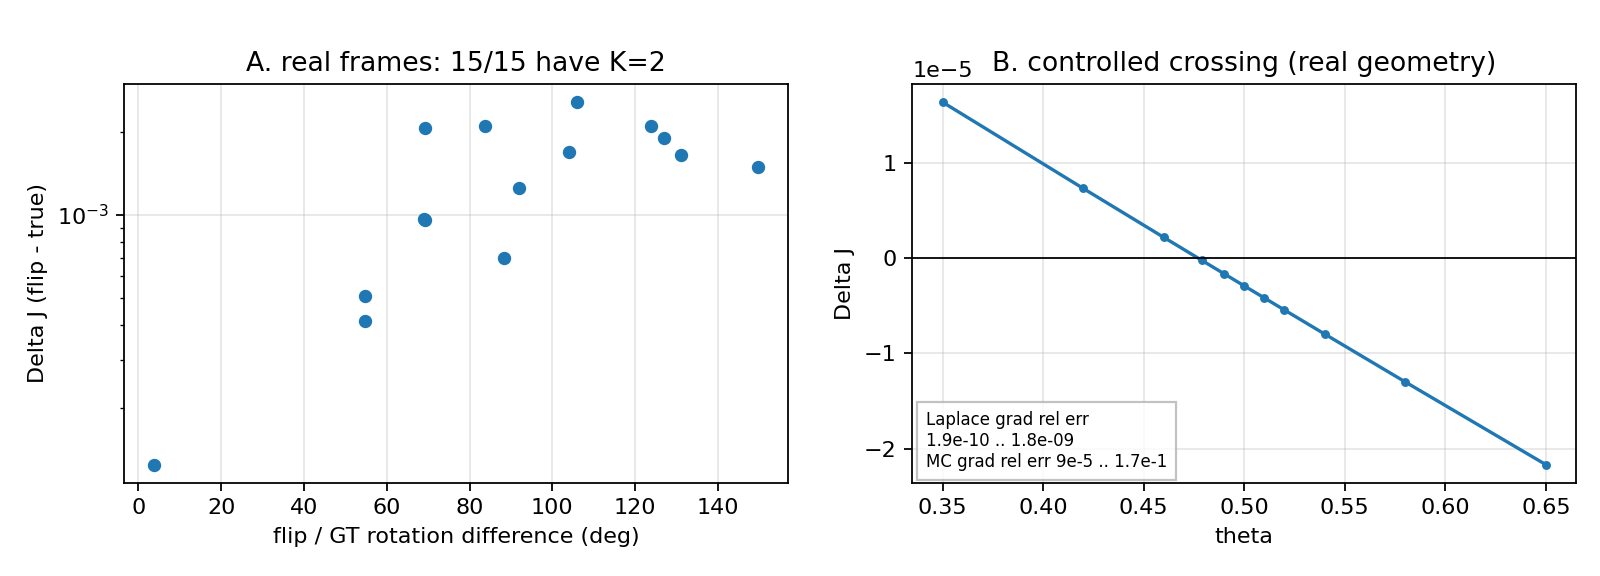
\includegraphics[width=\columnwidth]{two_mode.png}
\caption{真实双模态代价。左：$15$ 帧 LINEMOD 上，翻转模态与类真值模态的目标间隙 $\Delta J$ 对两模态夹角；每帧均有 $K_{\rm phys}=2$，$\Delta J\in[1.25\times10^{-4},2.56\times10^{-3}]$。右：真实几何上的受控横向交叉（B 部分），两个带标签假设按 $J_\theta=(1-\theta)J_{\rm true}+\theta J_{\rm sym}$ 混合；$\Delta J$ 在 $\theta\approx0.475$ 附近变号。插图为解析 Laplace 梯度相对中心 FD 的误差（$1.9\times10^{-10}$--$1.8\times10^{-9}$）与 $400$ 样本 MC 误差（$9\times10^{-5}$--$1.7\times10^{-1}$）。}
\label{fig:twomode}
\end{figure}

由此可得三点。第一，双模态结构可复现：$15/15$ 帧均有 $K_{\rm phys}=2$，$\Delta J\in[1.25\times10^{-4},2.56\times10^{-3}]$，另一模态夹角 $3.8^\circ$--$149.6^\circ$，$w({\rm other})=0.450$--$0.608$。第二，类真值模态在 $14/15$ 帧中是最低 $J$ 的物理模态，故硬 argmin 在这些帧上准确：旋转误差中位数 $2.06^\circ$ $[1.47,3.49]$，ADD-S 中位数 $3.7$ mm $[3.0,4.3]$，只有一帧误差超过 $10^\circ$（\texttt{000010/72}，$44.5^\circ$）。第三，Laplace 后验均值在这些近打平处并非精度提升：投影旋转误差中位数 $44.24^\circ$ $[33.90,46.87]$，相对硬 argmin 的成对偏差 $+36.9^\circ$ $[+27.2,+44.9]$，ADD-S 中位数 $13.9$ mm $[10.3,20.2]$，即约一半质量落在翻转模态。该集合中最小的 Hessian 行列式为 $6.09\times10^{-3}$（\texttt{000011/20}），故翻转模态本身接近折叠。

\begin{table*}[t]
\centering
\caption{$15$ 帧真实数据上的聚合位姿误差与 ADD-S。中位数及帧上 $95\%$ 百分位 bootstrap 置信区间（$1000$ 次重采样）。成对偏差为相对硬 argmin 的逐帧差均值（帧上 $95\%$ 置信区间）；成对旋转偏差中位数为 $+41.8^\circ$。“$\le10^\circ$”统计估计与真值相差不超过 $10^\circ$ 的帧数；对后验均值而言这并不等于“真模态”，因为均值未必是模态。}
\label{tab:aggregate}
\scriptsize
\setlength{\tabcolsep}{3.5pt}
\begin{tabular}{@{}l l l l l l l@{}}
\toprule
方法 & 旋转中位(°) & ADD-S 中位(mm) & ADD 中位(mm) & 旋转偏差(°) & ADD-S 偏差(mm) & $\le10^\circ$ / 真模态\\
\midrule
硬 argmin & 2.06 [1.47, 3.49] & 3.7 [3.0, 4.3] & 5.9 [5.2, 11.1] & --- & --- & 14/15 真模态\\
Laplace（投影） & 44.24 [33.90, 46.87] & 13.9 [10.3, 20.2] & 38.1 [31.0, 41.5] & +36.9 [+27.2, +44.9] & +9.4 [+6.4, +12.6] & 0/15\\
MC（20 种子） & 43.80 [33.90, 47.43] & 14.1 [10.3, 20.0] & 38.0 [31.0, 41.5] & +37.2 [+26.7, +45.0] & +9.4 [+6.4, +12.5] & 0/15\\
\bottomrule
\end{tabular}
\end{table*}

\begin{figure*}[t]
\centering
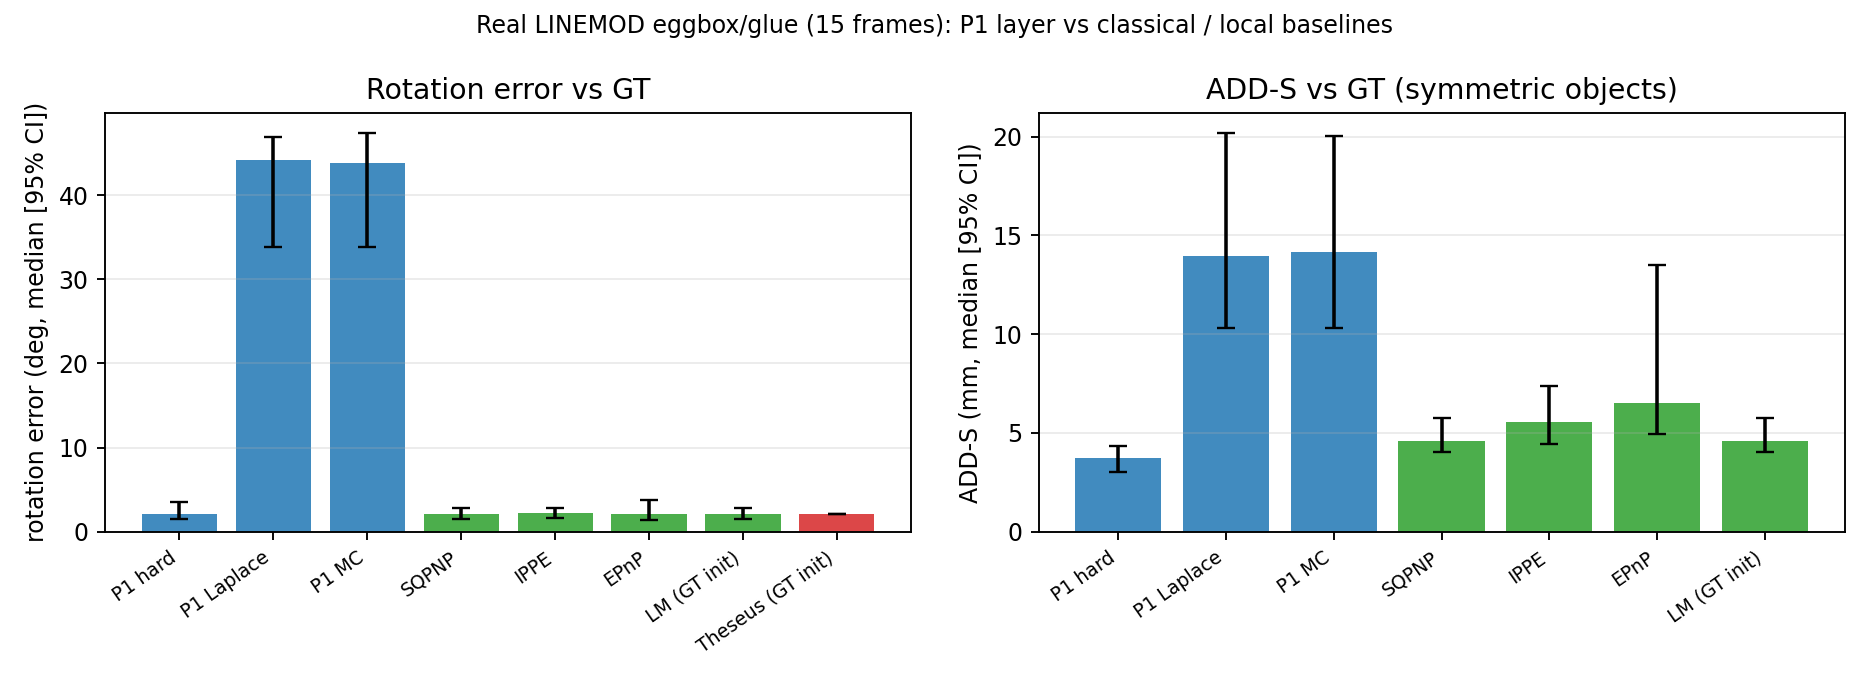
\includegraphics[width=\textwidth]{real_summary.png}
\caption{$15$ 帧真实 LINEMOD \texttt{eggbox}/\texttt{glue} 结果，中位数及 $95\%$ bootstrap 置信区间。左：P1 层（硬 argmin、投影 Laplace 均值、$20$ 种子 MC）与正演/局部参考（SQPNP、IPPE、EPnP、真值初始化的局部 LM、真值初始化的 Theseus）相对 BOP 真值的旋转误差。右：相同方法的 ADD-S（Theseus 未绘出）。硬 argmin 处于经典求解器水平；两个后验均值估计因对两个模态取平均而位于 $44^\circ$ 附近。绿色为前向/局部参考；红色为从真值初始化的局部求解器，不是可部署基线。}
\label{fig:realsummary}
\end{figure*}

$15$ 帧聚合结果见表~\ref{tab:aggregate}。硬 argmin 的均值大于中位数（$5.28^\circ$、$6.0$ mm），原因是个别失败帧；Laplace 的均值为 $42.21^\circ$ 与 $15.5$ mm；平移中位数为 $6.2$ mm（硬）与 $20.2$ mm（Laplace）。MC 估计与 Laplace 相同的平滑均值（$20$ 个种子均值的平均与 Laplace 聚合相差 $0.23^\circ$，在其种子级置信区间内），因此继承该偏差，只额外引入种子噪声（种子间标准差 $1.011^\circ$）。

\begin{table}[t]
\centering
\caption{$15$ 帧真实数据的逐帧 ADD-S（mm；表中“硬/Lap/MC”三列）与 ADD 参考（mm）。“ADD-S 是主要物体空间度量；ADD 为同索引距离，对物体的 $\sim180^\circ$ 对称性不变。}
\label{tab:perframe}
\scriptsize
\setlength{\tabcolsep}{2.5pt}
\begin{tabular}{@{}l r l l l l@{}}
\toprule
帧/图像 & 物体 & 硬 & Lap & MC & ADD（参考）\\
\midrule
000010/15 & 10 & 3.0 & 10.3 & 10.3 & 31.0\\
000010/18 & 10 & 4.3 & 12.2 & 12.3 & 37.6\\
000010/40 & 10 & 6.2 & 9.7 & 9.7 & 31.1\\
000010/60 & 10 & 3.0 & 13.9 & 14.1 & 40.7\\
000010/66 & 10 & 2.7 & 12.1 & 12.0 & 38.0\\
000010/72 & 10 & 12.5 & 8.4 & 8.4 & 22.3\\
000010/80 & 10 & 3.8 & 8.8 & 8.9 & 24.1\\
000010/90 & 10 & 3.1 & 8.5 & 8.4 & 23.3\\
000011/20 & 11 & 13.8 & 22.9 & 22.8 & 72.7\\
000011/24 & 11 & 2.8 & 20.2 & 20.0 & 40.5\\
000011/26 & 11 & 3.7 & 17.6 & 17.5 & 38.1\\
000011/32 & 11 & 3.1 & 19.0 & 19.0 & 41.5\\
000011/33 & 11 & 3.8 & 23.4 & 23.7 & 41.5\\
000011/40 & 11 & 2.2 & 16.8 & 16.7 & 44.7\\
000011/49 & 11 & 22.4 & 28.1 & 28.2 & 75.9\\
\bottomrule
\end{tabular}
\end{table}

逐帧结果有两点值得注意。(i) 在 \texttt{000010/72} 上，硬 argmin 是距真值 $44.5^\circ$ 的模态，而类真值模态距真值 $3.8^\circ$，但 $J$ 高出 $1.25\times10^{-4}$；Laplace/MC 落在两模态之间（$23.0^\circ$、$8.4$ mm），比硬失败更接近真值。这是损失排序在单帧上的偶然，不说明后验均值总体上更准确。(ii) Laplace 位姿的 ADD 是 ADD-S 的 $2$--$3$ 倍（中位数 $38.1$ 对 $13.9$ mm），因为 glue 物体细长，$\sim180^\circ$ 对称性会将其重标；这正是采用 ADD-S 而非 ADD 的原因。

\subsubsection{相同对应点上的经典前向求解器}\label{sec:classical}

表~\ref{tab:classical} 在逐位相同的 $15$ 帧对应点上运行 cv2 的 EPnP、ITERATIVE、SQPNP、IPPE，以及同一方位代价上的普通局部 GN/LM（两个研究已验证逐位一致；真值位姿重投影残差中位数为 $1.47$ px，即约 $1$ px 的最近顶点量化）。这些是前向求解器而非可微层：该 LM 是同一代价上的普通前向优化器，不是 BPnP，也不对其作任何梯度断言。IPPE 在投影到拟合平面的 RANSAC 内点上运行（它要求严格共面，平面性 RMS 为 $0.83$--$1.47$ mm）；其余求解器使用原始内点。

\begin{table*}[t]
\centering
\caption{$15$ 帧真实数据上的经典前向 PnP 基线。中位数及帧上 $95\%$ bootstrap 置信区间（$2000$ 次重采样）。“真模态”统计与真值相差 $10^\circ$ 以内的解。cv2 5.0.0 中 SQPNP 返回单一解（文档针对非 P3P/IPPE 标志，且在全部 $15$ 帧上观测到）；IPPE 返回两个平面解，其中第一个（重投影代价最小）在全部 $15$ 帧上都更接近真值，故 oracle 行与“IPPE 第一个”相同。}
\label{tab:classical}
\scriptsize
\setlength{\tabcolsep}{4pt}
\begin{tabular}{@{}l l l l@{}}
\toprule
方法 & 旋转中位[CI](°) & ADD-S 中位[CI](mm) & 真模态\\
\midrule
EPnP & 2.05 [1.41, 3.71] & 6.5 [5.0, 13.5] & 12/15\\
ITERATIVE（单应初始化 + LM） & 2.07 [1.60, 3.54] & 6.5 [5.7, 8.7] & 11/15\\
SQPNP（单一解） & 2.04 [1.47, 2.77] & 4.6 [4.0, 5.8] & 15/15\\
IPPE（第一个，平面投影） & 2.21 [1.68, 2.76] & 5.5 [4.4, 7.4] & 15/15\\
局部 LM，单位初始化 & 106.01 [69.14, 179.82] & 40.7 [28.0, 1708.7] & 3/15\\
局部 LM，真值初始化 & 2.06 [1.47, 2.77] & 4.6 [4.0, 5.8] & 15/15\\
局部 LM，翻转初始化 & 88.39 [69.08, 106.01] & 23.5 [16.9, 28.0] & 0/15\\
\bottomrule
\end{tabular}
\end{table*}

此处的 ADD-S 列使用 $1000$ 查询/$1000$ 真值顶点估计器，相对表~\ref{tab:aggregate} 的稠密真值 ADD-S 带有 $+1.1$ mm 离散化下限；两列不可直接比较，旋转误差才是可比的精度列。

由此可得三点。(i) 前向点精度处于经典水平：SQPNP/EPnP/ITERATIVE 中位数为 $2.04$--$2.07^\circ$，IPPE 为 $2.21^\circ$，在帧噪声内与硬 argmin 的 $2.06^\circ$ 相当；没有经典求解器接近 Laplace 均值的 $44.2^\circ$。(ii) 单解求解器在某些帧上自信地出错：EPnP 在 $3/15$ 帧、ITERATIVE 在 $4/15$ 帧上偏离真值超过 $10^\circ$（第四帧 \texttt{000011/20} 为 $10.0^\circ$，恰在阈值）；在 \texttt{000010/72} 上两者都返回 $44.3^\circ$/$44.0^\circ$ 的平面翻转解，重投影残差 $0.78$--$0.79$ px，而该翻转解在原始内点上甚至具有更低的方位代价。(iii) 如果没有 $z>0$ 物理性过滤与多起点，局部 LM 从单位初始化失败（$3/15$ 为真，$7/15$ 落到相机后方；中位数 $106^\circ$），从翻转初始化也无法进入真模态（$0/15$）；只有真值初始化能恢复。物理性过滤与枚举在该代价上确实起作用。

\subsubsection{同一代价上的 Theseus LM}\label{sec:theseus}

Theseus 0.2.3（\texttt{LevenbergMarquardt}，float64 CPU）最小化同一方位代价 \cite{pineda2022theseus}；其目标与 numpy 参考一致到 $1.1\times10^{-13}$，解析 Jacobian 与中心差分一致到 $1.3\times10^{-10}$。它是局部优化器：每次调用返回一个位姿，不识别枚举模态集，不返回后验，也不施加 $z>0$ 物理性过滤。

\begin{table*}[t]
\centering
\caption{真实方位代价上的 Theseus LM。“真模态”为与真值相差 $10^\circ$ 以内。随机初始化行在 $15$ 帧上各用 $20$ 个初始化（$300$ 次求解）；多起点行在 $5$ 个代表性帧上各用 $8$ 个初始化（$40$ 次求解），其中位数针对这 $40$ 次试验误差，而非 best-of-8 聚合。}
\label{tab:theseus}
\footnotesize
\setlength{\tabcolsep}{4pt}
\begin{tabular}{@{}l l l p{7.4cm}@{}}
\toprule
协议 & 旋转中位(°) & 真模态 & 结果分解\\
\midrule
真值初始化（15 帧） & 2.06 & 15/15 & 收敛到最近的 P1 模态（\texttt{000010/72} 上为 $3.8^\circ$ 模态，而非全局 argmin）\\
单位初始化（15 帧） & 178.82 & 1/15 & 6 次翻转、8 次其他；8 次在相机后方\\
每帧 20 个随机初始化（300 次求解） & 123.91 & 100/300 (33.3\%) & 57 次翻转、143 次其他、134 次非物理\\
8 初始化 $\times$ 5 帧（40 次求解） & 4.95 & 11/40 (27.5\%) & 无聚合后验；逐试验误差\\
\bottomrule
\end{tabular}
\end{table*}

真值初始化行是局部收敛，而非基线优势。冷启动时 Theseus 返回下降所进入的任一盆地——常是翻转模态或无约束代价的相机后方驻点，正是本文层枚举所剔除的解。它是该近打平代价上自然的无枚举参考，而不是 Laplace 均值的估计器；局部优化在此不能替代模态枚举。

\subsubsection{真实几何上的受控横向交叉}\label{sec:partb}

B 部分消除了早期构造的共享平移问题：两个带标签假设各自消去\emph{自己的}平移，代价按 $J_\theta=(1-\theta)J_{\rm true}+\theta J_{\rm sym}$ 混合。在真实帧 \texttt{000010/15} 上，实测打平点为 $\theta^\star\approx0.475$（构造设计为 $0.5$ 处打平，但重采样使两个带标签代价并非严格对称）；$\Delta J$ 在 $\theta=0.46$ 与 $0.479$ 之间变号，故交叉是横向的，两个极小保持在各自标签位姿的 $\sim2^\circ$ 以内。

\begin{table}[t]
\centering
\caption{真实几何上的受控横向交叉（B 部分，摘录）。\emph{梯度相对误差} 为解析 Laplace 梯度相对层输出中心 FD 的误差；MC 为 $400$ 样本的模态级估计。}
\label{tab:partb}
\scriptsize
\setlength{\tabcolsep}{2.5pt}
\begin{tabular}{@{}l l l l l l@{}}
\toprule
$\theta$ & $\Delta J$ & $w(A)$ & Lap 梯度 & MC 梯度 & $\|d\phi\|$\\
\midrule
0.3500 & +1.64e-05 & 0.50031 & 2.59e-10 & 9.51e-03 & 1.129e-02\\
0.4600 & +2.20e-06 & 0.50004 & 8.61e-10 & 8.94e-05 & 1.123e-02\\
0.4790 & -2.22e-07 & 0.50000 & 7.82e-10 & 1.68e-01 & 1.122e-02\\
0.5000 & -2.89e-06 & 0.49995 & 1.76e-09 & 5.09e-02 & 1.121e-02\\
0.6500 & -2.17e-05 & 0.49960 & 4.03e-10 & 1.10e-02 & 1.112e-02\\
\bottomrule
\end{tabular}
\end{table}

在全部 $11$ 行上，Laplace 梯度与中心 FD 一致到 $1.9\times10^{-10}$--$1.8\times10^{-9}$，而 $400$ 样本模态级 MC 误差为 $8.9\times10^{-5}$--$1.7\times10^{-1}$；硬 argmin 在打平处跳变，其 FD 无定义，故不报告硬梯度。这是闭式反向传播在真实代价上的正确性结果；ADD-S 代理属于 A 部分。

\subsection{运行时间与批处理}\label{sec:compute}

\textbf{仅 CPU。} 所有报告运行均为单进程 CPU 作业。SDP 运行使用 cvxpy 1.9.3/SCS（$\varepsilon=10^{-9}$，\texttt{max\_iters=200000}），对比实验使用 cvxpy 1.7.5/SCS，六点检验使用 $\varepsilon=10^{-11}$、\texttt{max\_iters=10\textasciicircum 6} 的 SCS。真实数据与根计数为短时 CPU 作业：位姿误差/ADD-S 约 $10$ s，经典基线 $3.0$ s，Theseus 对比 $9.5$ s，四个实例的根计数约 $30$ s。

\textbf{计时。} 由 $20$ 次重复，$\theta=0$ 处一次完整合成层调用中位数为 61.9 ms（p95 62.1）：模态枚举占 $88\%$，$K$ 次隐式 $3\times3$ 求解占 $1.6\%$，解析反向（权重梯度与混合）占 $0.1\%$。$\theta=-0.1$ 时整次调用为 17.7 ms。LINEMOD 每帧前向为 24.2--265.9 ms，横向交叉每个 $\theta$（含 FD）为 33.1--42.6 ms。

\textbf{批处理。} 真正的批量多起点 Newton 在批大小 64 时仅比循环快 $1.30\times$（59.9 对 46.2 样本/秒），批大小 8 时为 $0.78\times$，为 1 时为 $0.46\times$：收敛异质性与逐实例分类循环占主导，故需要 GPU 或定制内核才能获得实际吞吐收益。瓶颈是模态枚举，而非 $3\times3$ 求解。
